\documentclass[border=6pt]{standalone}
\usepackage[T1]{fontenc}
\usepackage[utf8]{inputenc}
\usepackage{mathptmx}
\usepackage{amsmath,amssymb,amsfonts,mathrsfs}
\usepackage[dvipsnames]{xcolor}
\usepackage{tikz}
\usetikzlibrary{calc,positioning,arrows.meta,decorations.pathreplacing,
                decorations.markings,matrix,fit,backgrounds,shapes.misc}
\renewcommand{\sl}{\mathfrak{sl}}
\newcommand{\Uq}{U_q(\sl_2)}
\newcommand{\qint}[1]{[#1]_q}
\newcommand{\Rcheck}{\check{R}}
\definecolor{accent}{RGB}{59,91,146}
\definecolor{accentsoft}{RGB}{155,180,216}
\definecolor{oddsign}{RGB}{138,40,132}
\tikzset{
  strand/.style={line width=1pt, accent!80!black},
  rbox/.style={draw=accent!70!black, fill=accentsoft!55, rounded corners=2pt,
               line width=0.8pt, minimum height=6mm},
  rdot/.style={circle, fill=accent, inner sep=1.6pt},
  knode/.style={circle, draw=accent!70!black, fill=accentsoft!45,
                line width=0.8pt, minimum size=7mm, font=\small},
  kedge/.style={accent!70!black, line width=0.9pt},
  faredge/.style={oddsign!75!black, line width=0.9pt, densely dashed},
  glabel/.style={font=\footnotesize, accent!60!black},
}
\begin{document}
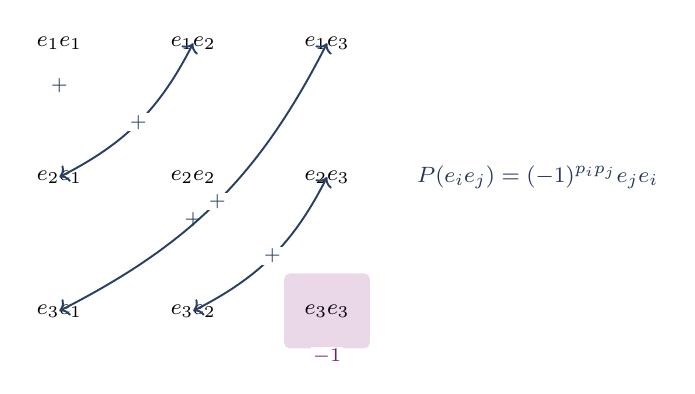
\begin{tikzpicture}[x=1.7cm,y=1.7cm]
  % 3x3 baz izgarasi: hucre (i,j) -> e_i e_j
  \foreach \i in {1,2,3}{
    \foreach \j in {1,2,3}{
      \coordinate (c\i\j) at (\j, -\i);
    }
  }
  % odd-odd hucresi (3,3) vurgulu
  \fill[oddsign!18, rounded corners=2pt] (3-0.32,-3-0.28) rectangle (3+0.32,-3+0.28);
  \foreach \i in {1,2,3}{
    \foreach \j in {1,2,3}{
      \node[font=\footnotesize] at (c\i\j) {$e_{\i}e_{\j}$};
    }
  }
  % kosegen-disi takas oklari (+1)
  \foreach \i/\j in {1/2,1/3,2/3}{
    \draw[<->, accent!70!black, line width=0.7pt]
      (c\i\j) to[bend left=18] node[font=\scriptsize, fill=white, inner sep=0.6pt] {$+$} (c\j\i);
  }
  % kosegen sabit (isaret)
  \node[font=\scriptsize, accent!60!black] at (1+0.0,-1-0.32) {$+$};
  \node[font=\scriptsize, accent!60!black] at (2+0.0,-2-0.32) {$+$};
  \node[font=\scriptsize, oddsign!80!black, fill=white, inner sep=0.6pt] at (3,-3-0.34) {$-1$};
  \node[glabel, accent!60!black, anchor=west] at (3.6,-2)
    {$P(e_ie_j)=(-1)^{p_ip_j}e_je_i$};
\end{tikzpicture}
\end{document}
